\chapter{Preliminaries}

In this chapter a simple model will explain the relation between power harvested and distance covered by the robot.
The design considerations for the robot will be explained based on minimal required capabilities. 
Followed by an evaluation of stepper motor based locomotion for a transiently powered robot.

\section{Transiently-powered Actuation Model}
\label{sec:transient_model}

% 1 Incomming power V * I which scales with solar panel size

% 2 Maximum power point tracking (switchmode boost converter)

% 3 Stored in non-ideal supercapacitor with capcitiy C and a parrallel resistance Rleak and series resistance (ESR, typically small but not neglectable?)

% 123 determine chargetime

% Buck converter losses 

% Power consumed from source = Pcons = Ploss + Pweels

% Power P(t)  = F * v = T x omega


% robot dynamics model

%\begin{equation}
%	F_{r} = \mu_{r} F_{N} = \mu_{r} mg
%\end{equation}

%\begin{equation}
%F_{a} = \frac{1}{2}\rho v^2C_{d}A
%\end{equation}


\section{Design Considerations}
\label{sec:design_considerations}

This section will shortly explain the main areas considered while designing the battery-less transiently-powered robot

% - Optimize or low power consumption (disable or standby sensors and motor ctrl when not used)
% - Minimal basic functionality (for simple swarm algorithms?) (but no power hungry components ie optical encoders or mouse sensors)
% - Low power communication
% - Navigation

% Extra extra:
% - Tradeoff chargetime and operation time

\begin{enumerate}
\item \textbf{Power} The robot should not rely on batteries, alternatively energy can be harvested from ambient sources and stored in a supercapacitor. 
Energy harvested in a controlled environment should charge the capacitor in under 10 seconds and stored energy should provide at least an operation time of 1 second, allowing the robot to make short controlled movements.

\item \textbf{Small form factor} By making the robot as small as possible, weight is kept to a minimum reducing the energy required for movement.
Secondly, by designing the robot to use low cost regular available parts should future proof the robot for use in a transiently-powered swarms.

\item \textbf{Locomotion}
The energy used for movement will be the biggest part used from the total available energy budget.
To optimize the distance that can be covered with a single capacitor charge, an efficient locomotion type should be chosen for the movement on flat surfaces.

\item \textbf{Autonomous navigation}
During operation the robot will experience a very frequent loss of power. 
Despite regular power interruption the transiently-powered robot should be able to complete a movement with an acceptable error compared to the same robot being battery powered. 

\end{enumerate}


% RF harvesting seems prommesing
% Wispcam requires approx 4 seconds to harvest 20mJ at a distance of 20cm from the reader \cite{naderiparizi_rfid_2015}
% better to only use RF for communication and harvest energy from another source \cite{konstantioulos}

% Energy can be harvested from different sources

\section{Stepper motor-based Locomotion}

Autonomous navigation requires robot to have accurate locomotion and basic odometry.
On bigger robots wheel encoders are commonly used to determine the angular speed of each wheel, used for controlling movement and odometry.
Miniaturizing encoders significantly reduces their resolution, and can be classified as power hungry when considering a small energy budget and active light source is used.
The GRITSBot uses stepper motors to achieve accurate locomotion and basic odometry, as described in Section \ref{sec:locomotion}.
This section will further investigate the use of stepper motor based locomotion in combination with a transiently-powered robot.

\subsection{The Stepper Motor}
Stepper motors are a type of permanent magnet dc motor that start to rotate by supplying current to the motor coils in a specific direction.
The bipolar stepper motor used, requires current to be pulsed trough each of the four connections, in a fixed pattern, in order to rotate it forward or backward.
A Microcontroller (MCU) is used to keep track and instruct the next stepper motor position from a sequence of four.
The outputs of the MCU cannot supply enough current to drive a bipolar stepper motor, therefore a dual H-bridge is required to control the current trough each coil.

%TODO make new schematic stepper figure!
%http://homemaderobo.blogspot.nl/2012/03/stepper-motor.htm
\begin{figure}
	\centering
	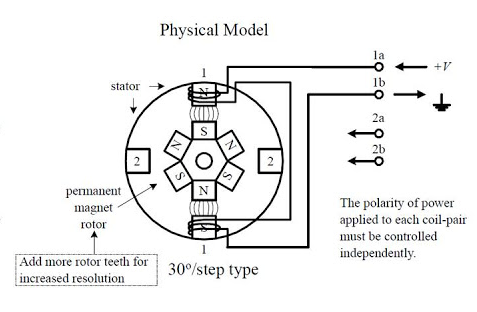
\includegraphics[width=\textwidth]{pics/bipolar_stepper.png}
	\caption{Need better / simpler figure here!}
	\label{fig:bipolarstepper}
\end{figure}

\subsection{Control and Rotor Synchronization}

The only way to grantee that the teeth on the rotor will stay aligned with the coil is to keep the coil energized until the next position is instructed and the other coil is energized. 
On the first startup it can happen that the rotor is not aligned with the last position in the sequence.
When this happens there can be an error between one and three steps of instructing a new steps and the stepper moving to the next position.

In case the stepper motor is rotating and the power is removed, misalignment between the rotor and the last energized coil can occur.
While the rotor could be moving from one position to the next, it has not moved at all (undershoot) or it overshoots it's next position due to inertia of the rotating mass. 
To determine what would be more likely, undershooting or overshooting, an experiment has been preformed to determine the error in number of steps.

\subsection{Experimental setup}

A stepper motor is suspended and a needle glued to the motor shaft.
The needle rotates over a round piece of paper which is divided by markings every 18 degrees, as can be seen from Figure \ref{fig:step_counting}.
First the rotor and coil is synchronized by moving 4 steps.
Then the position of the needle is recorded and the stepper motor is commanded to make one rotation equal to 20 steps.
After rotating 20 steps the power is removed and the needle position recorded when the needle is not rotating anymore.

\begin{figure}
	\centering
	\begin{subfigure}[b]{0.38\textwidth}
		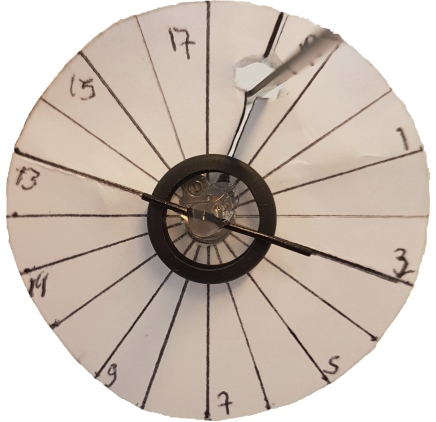
\includegraphics[width=\textwidth]{pics/step_counting.jpg}
		\caption{Experimental setup for determining error in the number of counted steps}
		\label{fig:step_counting}
	\end{subfigure}
	\quad
	\begin{subfigure}[b]{0.55\textwidth}
		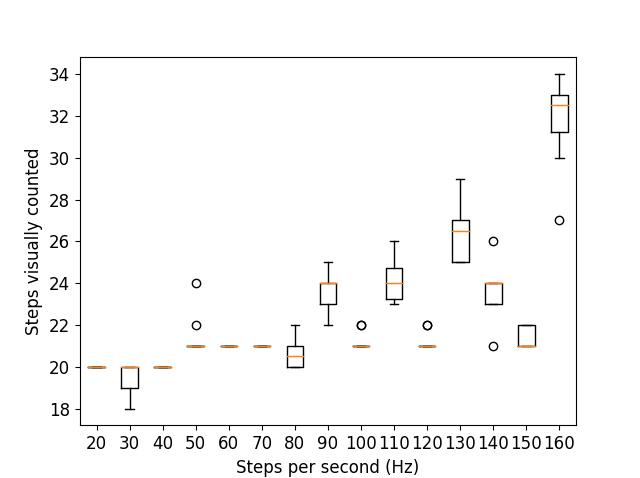
\includegraphics[width=\textwidth]{pics/figure_intertia.png}
		\caption{}
		\label{fig:step_results}
	\end{subfigure}
	\caption{}
\end{figure}

\subsection{Result}

% Differential drive robot using two stepper motors has a 

%The current trough the coils is constant, so the faster the stepper motor changes step the more energy can be transformed into movement.
%Increasing the rotational speed of the stepper motor decreases the torque output of the motor.
%Therefore the speed is limited by the amount of torque required to preform the movement.





